\documentclass[titlepage,12pt,a4paper,times]{book}
\usepackage{soul}
\usepackage[utf8]{inputenc}
\usepackage[portuguese]{babel}
\usepackage[T1]{fontenc}
% substituir linha anteior por 
% \usepackage[english]{babel} 
% se o relatório for escrito na língua inglesa.
\usepackage{makeidx}
\usepackage{xspace}
\usepackage{graphicx,color,times}
\usepackage{fancyhdr}
% \usepackage{pxfonts}
% \usepackage{times}
% \usepackage{mathptm}
% \usepackage{amssymb}
% \usepackage{amsfonts}
\usepackage{amsmath}
\usepackage{latexsym}
\usepackage[printonlyused]{acronym}
\usepackage{float}
\usepackage{listings}
\usepackage{listing}
\usepackage{tocbibind}
\usepackage{wrapfig}
\usepackage{natbib}
\usepackage[hyphens]{url}
\usepackage{hyperref}


% \usepackage{glossaries}
% \makeglossaries


\renewcommand{\ttdefault}{phv}

\pagestyle{fancy}
\renewcommand{\chaptermark}[1]{\markboth{#1}{}}
\renewcommand{\sectionmark}[1]{\markright{\thesection\ #1}}
\fancyhf{} \fancyhead[LE,RO]{\bfseries\thepage}
\fancyhead[LO]{\bfseries\rightmark}
\fancyhead[RE]{\bfseries\leftmark}
\renewcommand{\headrulewidth}{0.5pt}
\renewcommand{\footrulewidth}{0pt}
\addtolength{\headheight}{0.5pt}
\setlength{\marginparsep}{0cm}
\setlength{\marginparwidth}{0cm}
\setlength{\marginparpush}{0cm}
\addtolength{\hoffset}{-1.0cm}
\addtolength{\oddsidemargin}{\evensidemargin}
\addtolength{\oddsidemargin}{0.5cm}
\addtolength{\evensidemargin}{-0.5cm}


% NEW COLORS
\definecolor{dark}{gray}{0.25}
\definecolor{lgray}{gray}{0.9}
\definecolor{dkblue}{rgb}{0,0.13,0.4}
\definecolor{dkgreen}{rgb}{0,0.6,0}
\definecolor{gray}{rgb}{0.5,0.5,0.5}
\definecolor{mauve}{rgb}{0.58,0,0.82}

\lstset{ %
  language=java,                    basicstyle=\footnotesize,
  numbers=none,                  numberstyle=\tiny\color{gray}, 
  stepnumber=1,                  numbersep=5pt,
  backgroundcolor=\color{white}, showspaces=false,
  showstringspaces=false,        showtabs=false,
  frame=single,                  rulecolor=\color{black},
  tabsize=2,                     captionpos=b,
  breaklines=true,               breakatwhitespace=false,
  title=\lstname,                keywordstyle=\color{blue},
  commentstyle=\color{dkgreen},  stringstyle=\color{mauve},
  escapeinside={\%*}{*)},        morekeywords={*},
  belowskip=0cm
}



\begin{document}


\thispagestyle{empty}
\setcounter{page}{-1}

\begin{center}
\begin{Huge}
\textbf{Universidade da Beira Interior}
\end{Huge}
\end{center}

\begin{center}
\begin{Huge}
Departamento de Informática
\end{Huge}
\end{center}

\vspace{0,07cm}
\begin{figure}[!htb]
\centering
\includegraphics[scale=0.3]{brasãoubi.jpg}
\end{figure}

\vspace{0.5cm}
\begin{center}
\begin{Large}
\textbf{Batalha Naval - TankUP}\\
% * <individuoamaral@gmail.com> 18:56:55 10 Apr 2017 UTC+0100:
% confirmar nome do jogo
Relatório Técnico
\end{Large}
\end{center}

\vspace{0.3cm}
\begin{center}
\begin{normalsize}
\begin{large}
Discente:
\end{large}
\end{normalsize}
\end{center}

\vspace{0.2cm}
\begin{center}
\begin{large}

\textbf{João Amaral - 33692}\\

\end{large}
\end{center}

\vspace{0,4cm}
\begin{center}
\begin{normalsize}
\begin{large}
Cadeira:
\end{large}
\end{normalsize}
\end{center}

\vspace{0.2cm}
\begin{center}
\begin{large}
\textbf{Projeto}\\
\end{large}
\end{center}

\vspace{0,4cm}
\begin{center}
\begin{normalsize}
\begin{large}
Docente:
\end{large}
\end{normalsize}
\end{center}

\vspace{0.2cm}
\begin{center}
\begin{large}
\textbf{Professor Doutor Frutuoso Silva}
\end{large}
\end{center}


\vspace{0.4cm}
\begin{center}
\begin{normalsize}
17 de Julho de 2017

\end{normalsize}
\end{center}


\clearpage{\thispagestyle{empty}\cleardoublepage}

\frontmatter

\clearpage{\thispagestyle{empty}\cleardoublepage}


\tableofcontents

\clearpage{\thispagestyle{empty}\cleardoublepage}

\listoffigures

% Se não existirem tabelas, comentar as seguintes linhas
\clearpage{\thispagestyle{empty}\cleardoublepage}
\listoftables

\clearpage{\thispagestyle{empty}\cleardoublepage}
\chapter{Acrónimos}
\label{chap:acro}

\begin{acronym}[TCP]
    \acro{TCP}{Transmission Control Protocol}
\end{acronym}

\begin{acronym}[IP]
    \acro{IP}{Internet Protocol}
\end{acronym}

\begin{acronym}[DLC]
    \acro{DLC}{Downloadable Content}
\end{acronym}

% \clearpage{\pagestyle{empty}\cleardoublepage}
% \include{glossario}
\chapter{Agradecimentos}
\label{chap:agradecimentos}

Gostava de agradecer aos meus pais, Agostinho Amaral e Teresa Aguiar, por sempre me apoiarem e ajudarem em tudo, e por fazerem com que a minha licenciatura fosse possível. \\

À minha namorada Joana Pereira, por me ajudar, apoiar e motivar sempre que desanimava quando encontrava algum problema que não conseguia resolver. \\

Ao meu orientador, o Professor Doutor Frutuoso Silva, que me guiou e contribuiu para que este trabalho tivesse qualidade. Além de ser um bom professor, também foi um bom formador, dado que me deixou trabalhar na área que mais me interessava e ainda me orientou nela.\\

E claro, aos meus amigos, que me apoiaram, ajudaram com o que precisei, e me fizeram perceber que, na realidade, as lições mais valiosas que se aprendem na universidade não são numa sala de aulas. Agradeço especialmente à Maria Pissarra, ao José Santos, ao Luis Duarte, ao Rui Infante, ao José Manteigueiro, ao Guilherme Catalão, ao Nuno Queirós e ao Carlos Oliveira, por serem amigos incríveis e por me terem  animado, motivado e também criticado. \st{E também pelos memes}.
\clearpage{\thispagestyle{empty}\cleardoublepage}

\clearpage{\thispagestyle{empty}\cleardoublepage}


\mainmatter
\chapter{Resumo}
\label{chap:resumo}

\section{Introdução ao tema}
\label{resumo:sec:intro}
Este projeto consiste no desenvolvimento de um jogo multi-jogador para a plataforma Android, baseado no clássico jogo de tabuleiro da \emph{Batalha Naval}, consistindo num conflito, por turnos, de viaturas terrestres num mapa em grelha 4*4, colocadas e controladas por dois jogadores que não têm conhecimento do conteúdo do tabuleiro do jogador inimigo.


\section{Abordagem ao tema}
\label{resumo:sec:ATL}
Primeiramente, foi feita uma avaliação das plataformas móveis mais viáveis para a realização do projeto, sendo depois escolhida a sua arquitetura de rede (\textit{sockets} \ac{TCP}). Depois de definido o modo de comunicação, foram definidas as mecânicas de jogo e as regras de jogabilidade, de maneira a controlar o desenrolar do jogo de acordo com o pretendido. \\ 

Concluída a fase de planeamento e design, procedeu-se ao desenvolvimento dos \textit{assets} para implementação no jogo, tais como modelos 3D dos veículos, animações e produção de vídeos. Estando os assets findados, procedeu-se à implantação destes no motor de jogo bem como à criação de \textit{scripts} para os controlar. Na fase final foram feitos vários testes de usabilidade da aplicação.

O presente relatório tem vindo a ser elaborado desde o início do ciclo de desenvolvimento da aplicação.



\clearpage{\thispagestyle{empty}\cleardoublepage}
\chapter{Introdução}
\label{chap:intro}
\section{Considerações iniciais}
\label{sec:PBL} 
Este projeto foca-se na elaboração do jogo \textit{TankUP} para dois jogadores, multijogador, a partir da plataforma móvel Android. O objetivo do jogo consiste em destruir as viaturas do adversário, tentando adivinhar as suas posições e os seus respectivos  padrões de colocação.\\

O jogo teve como base o histórico “Batalha Naval”, contudo foram introduzidas algumas alterações de modo a tornar a experiência mais única e simples.
Este projeto não pretende a criação de um jogo com mecânicas, design ou gráficos de um jogo de topo atual, mas sim a exposição do estudo efetuado sobre como realizar um projeto utilizando tecnologias com as quais o autor não tinha qualquer experiência.\\
Em suma, o presente relatório focar-se-á no processo de aprendizagem e desenvolvimento do projeto, sendo encorajada a utilização da aplicação de modo a interagir mais dinamicamente com o relatório.



\section{Enquadramento do tema}
\label{sec:AIL}
Nesta secção serão expostas as abordagens iniciais em relação ao projeto no seu todo e às suas várias etapas.

A primeira abordagem ao projeto é relativa à pesquisa, onde foi estudado o ciclo normal de desenvolvimento de um videojogo e foram exploradas as ferramentas disponíveis neste mercado. Devido à complexidade do projeto, este envolve a maior parte do ciclo de desenvolvimento normal, sendo este o conceito, design, mecânicas, desenvolvimento e teste. \\ 

Servindo de base a proposta de projeto e tendo em conta este ciclo, começou-se por definir uma ideia mais concreta do pretendido. Depois, encontrar as ferramentas mais indicadas de utilizar em cada etapa. Isto foi conseguido pesquisando por vantagens que umas plataformas tinham em relação às outras e comparando trabalhos já desenvolvidos por autores mais experientes na área, usando fóruns e palestras disponibilizadas por vários estúdios de produção, como o \href{https://unite.unity.com/}{Unite}.

Depois de definir as ferramentas a utilizar, foi estudada a melhor maneira de implementar o jogo, definindo a sua arquitetura de rede, as suas características e funcionalidades base e que tipo de conteúdo poderia ser criado para este. 
Superada esta fase, houve o processo de aprendizagem das ferramentas e o desenvolvimento dos conteúdos gráficos. Foi então desenvolvido o jogo em si e testado, sendo que o desenvolvimento deste relatório foi acompanhando todo o processo.




\section{Motivação}
\label{sec:DP}
O objectivo desta aplicação consiste na aprendizagem e estudo das ferramentas utilizadas na indústria dos videojogos, dado o meu interesse pela área em questão. Dito isto, o desenvolvimento da aplicação serviu o seu propósito, sendo que, para a sua produção, foram utilizadas duas ferramentas frequentemente utilizadas na indústria - \emph{Blender} e \emph{Unity} - e foram aprofundados conhecimentos de ligações de rede, programação orientada a objetos, planeamento e de engenharia de \textit{software}. Foram também aprendidas novas técnicas e áreas da criação de videojogos como a modelação, animação, construção de cena e design de mecânicas de jogo.

Durante o desenvolvimento da aplicação, tornou-se claro que esta tinha um interesse que ia para além do espetro académico, no sentido em que poderia ser aproveitada para um projeto a ser inserido na indústria, ou seja, proceder à publicação do jogo numa plataforma de venda \textit{online} como a \emph{Play Store} da \emph{Google}. 
Mesmo não aplicando o conteúdo da aplicação para a construção do jogo, as suas capacidades poderiam ser aplicadas para outros projetos interessantes, como se pode verificar no \autoref{chap:futuroC}.

\section{Divisão do projeto}
\label{sec:DPL}
Para atingir uma mecânica ótima do desenvolvimento do projeto tornou-se de importante interesse a divisão do mesmo em várias fases e dentro destas várias tarefas, enumeradas da seguinte forma:
\begin{enumerate}
\item Definição do conceito base do jogo.\\

\item Avaliação das plataformas mais viáveis para a realização do projeto
\begin{enumerate}
\item Pesquisa de ferramentas de desenho e modelação.
\item Pesquisa de ferramentas de física e motor de jogo.\\
\end{enumerate}


\item Escolha da plataforma e arquitetura
\begin{enumerate}
\item Pesquisa sobre as diferentes escolhas de arquitetura disponíveis.
\item Pesquisa sobre as vantagens e limitações das ferramentas escolhidas ao implementar a arquitetura escolhida.
\item Escolha das ferramentas e arquitetura.\\
\end{enumerate}

\item Criação dos conteúdos do jogo
\begin{enumerate}
\item Aprendizagem da ferramenta \textit{Blender}.
\item Desenvolvimento dos modelos e vídeos a utilizar.\\
\end{enumerate}

\item Desenvolvimento do jogo
\begin{enumerate}
\item Aprendizagem da ferramenta \textit{Unity}.
\item Desenvolvimento das mecânicas e código do jogo.\\
\end{enumerate}

\item Fase de testes e refinação
\begin{enumerate}
\item Testes do jogo em diferentes máquinas e condições de rede.
\item Correção de erros e melhoramentos.\\
\end{enumerate}

\item Escrita de relatório.

\end{enumerate}

\clearpage

\section{Estrutura e organização do relatório}
\label{sec:ODL}

Este documento encontra-se estruturado da seguinte forma:
\begin{enumerate}
\item \autoref{chap:resumo} -- \textbf{Resumo} -- apresentação, de uma forma muito resumida, do tema, objetivos e abordagem seguida.

\item \autoref{chap:intro} -- \textbf{Introdução} -- enquadramento e  explicação do problema e a motivação, assim como, de grosso modo, a descrição da abordagem para a sua resolução.  De forma numerada, descreve-se a estrutura do relatório.

\item \autoref{chap:relacionados} -- \textbf{Estado de Arte} -- expostos trabalhos de caráter semelhante, servindo de inspiração ao desenvolver a aplicação.

\item \autoref{chap:tecnologias_ferramentas_utilizadas} -- \textbf{Tecnologias e Ferramentas Utilizadas} --  são abordadas as tecnologias e ferramentas utilizadas para desenvolver a aplicação.

\item \autoref{chap:desen} -- \textbf{Desenvolvimento} -- retrata-se todo o processo de desenvolvimento pela qual a aplicação passou. Descreve-se os detalhes de código e do projeto em geral, de maneira a fornecer uma ideia mais esclarecedora da estrutura base responsável para o funcionamento da aplicação. 

\item \autoref{chap:futuroC} -- \textbf{Conclusões e Trabalho Futuro} -- capítulo onde são enunciadas diferentes maneiras de melhorar o jogo, adicionando ou melhorando diferentes aspetos deste. Também é feito um resumo do que foi abordado anteriormente e são referidas algumas considerações sobre o projeto em si.

\end{enumerate}


\clearpage{\thispagestyle{empty}\cleardoublepage}
% \chapter{Decisões}
\chapter{Trabalhos Relacionados}
% OU \chapter{Engenharia de Software}
% OU \chapter{Tecnologias e Ferramentas Utilizadas}
\label{chap:relacionados}

\section{Introdução}
\label{chap2:sec:intro}
Este capítulo pretende mostrar e comparar algum trabalho já feito anteriormente, na mesma área que o TankUP, de maneira a esclarecer como e onde este se encaixa no ambiente existente. Neste sentido, primeiro é feito um \textit{overview} das características mais gerais do trabalho que foi feito, sendo depois comparado com alguns trabalhos relacionados.

\section{Resumo de Características Gerais}
\label{chap2:sec:DGL}
A seguir, é apresentada uma tabela que resume as características mais gerais da aplicação desenvolvida:
\begin{table}
\caption{Tabela de características gerais.}
\label{tab:tabela_caracteristicas_gerais}
\centering
\begin{tabular}{|c||l|l|}
\hline
\hline
\textbf{\#} & \textbf{Tecnologia} & \textbf{Escolha} \\
\hline
\hline
1 & Plataforma Móvel & \emph{Android} \\
\hline	
2 & Motor de Jogo & Unity3D \\
\hline
3 & Modelação 3D  & Blender\\
\hline
4 & Base do jogo &  Multi-Jogador por Turnos\\
\hline
5 & Linguagem de Programação & C\#\\
\hline
6 & Modelo de Arquitectura de Comunicação & Cliente - Servidor\\
\hline
7 & Modo de Comunicação & Sockets \ac{TCP}\\
\hline
\end{tabular}

\end{table}
\clearpage

\section{Fundamentação das Características Gerais}
\label{chap2:sec:DEL}
A seguir, vão ser explicadas as escolhas relativas às  características gerais supramencionadas, refletindo o  processo de criação em relação à aplicação.
% * <individuoamaral@gmail.com> 12:18:31 13 May 2017 UTC+0100:
% meter uma estatística de utilização no #1
\begin{enumerate}
\item Uma plataforma móvel que está a mostrar um crescimento exponencial em termos de utilização e público. Trata-se de uma plataforma flexível, sendo reconhecida, assim como o \emph{iOS} da \textit{Apple} [1], como as maiores plataformas de distribuição de jogos, atingindo um público avassalador [10]. Nestes termos, há mais de dois biliões de dispositivos móveis únicos a correr aplicações feitas em \emph{Unity} e tendo uma percentagem de trinta e quatro porcento do mercado de motores de jogo do mundo [17]. Têm-se presenciado inúmeros êxitos inesperados em jogos móveis de pequena dimensão (como é o caso com \textbf{Flappy Bird}), que servem para mostrar que a área tem um crescimento possivelmente exponencial, opinião suportada por outras pesquisas [8] [11] e que nascem várias oportunidades propícias a evolução. A escolha também foi feita devido à experiência  com a plataforma Android, vinda de projetos passados.

\item[2]  O motor de jogo escolhido para desenvolver a aplicação foi o \emph{Unity3D}. Este motor de jogo, além de ser grátis para projetos de pequena envergadura, já deu várias provas de como tem qualidade suficiente para ser utilizado por grandes estúdios de jogos e fazer projetos de sucesso. Poderia ter feito a aplicação utilizando a interface gráfica do Android nativo, no entanto, quis aproximar-me o mais possível do \textit{standard} da indústria. Não tinha qualquer experiência no uso desta ferramenta.

\item[3] A ferramenta de modelação usada para a criação dos \textit{assets} gráficos da aplicação foi o Blender, onde foram feitos os modelos do tanque, do jipe e da artilharia utilizados nos clipes de vídeo. Esta escolha foi feita, mais uma vez, com base no \textit{standard} da indústria [7], sendo uma ferramento profissional de renome, sendo utilizada por vários estúdios de sucesso. Não tinha qualquer experiência no uso desta ferramenta.

\item[4] O jogo consiste em dois tabuleiros 4*4, um para cada jogador, onde cada um vai colocar ao calhas seis peças, sendo que nenhum tem acesso ao tabuleiro do outro e, a única maneira de o adivinhar, é utilizando as respostas do jogo quando um jogador acerta em algo do jogador inimigo. A mecânica do jogo consiste numa batalha, por turnos, entre dois jogadores, na qual o objectivo é destruir o máximo dos veículos do outro jogador.

\item[5] A linguagem de programação escolhida para o projeto foi \emph{C\#} [13]. Mais uma vez, esta escolha foi feita com base no \textit{standard} da indústria. Para trabalhar com o motor de jogo \emph{Unity}, a linguagem de programação tem de ser ou \emph{C\#} ou \emph{JavaScript}. Escolhi \emph{C\#} dado a ter mais experiência em linguagens que entram no mesmo modelo que esta (\emph{Java}) do que com \emph{JavaScript}.

\item[6] Para o modelo de comunicação escolhi usar \emph{Cliente/Servidor}, dado ser o modo para o qual o \emph{Unity} oferece melhor suporte. Também havia interesse em explorar melhor os conceitos que formam a base deste modelo. Os restantes conceitos que foram estudados foram \textit{Bluetooth} [6] e \textit{Peer-to-peer} [3].

\item[7] Para o modo de comunicação, em vez de usar as ferramentas disponibilizadas pelo \emph{Unity}, tais como o seu \emph{NetClient} e módulo multijogador, foram utilizados \emph{Sockets \ac{TCP}} [12], dado que assim é possível aperceber-se, de uma forma mais detalhada, como a comunicação entre os clientes e o servidor é feita e qual a dimensão de dados que é preciso passar entre eles.
\end{enumerate}
\clearpage

\section{Projetos Relacionados}
\label{chap2:sec:PRL}
Para a planificação da aplicação, foram considerados dois projetos nos quais me baseei para, de uma maneira mais informada, me ambientar à elaboração da minha aplicação. Estes trabalhos foram: 
\begin{enumerate}
    \item \textbf{Battleship}\\
    De uma forma resumida, o jogo da Batalha Naval [2] consiste num jogo por turnos no qual dois jogadores colocam um determinado número de peças, de vários tipos, no seu tabuleiro sem o conhecimento do outro jogador.
    A cada turno, um jogador seleciona uma posição do tabuleiro do seu adversário para atacar e, caso acerte, tem de lhe ser comunicado por parte do adversário. O jogador que conseguir acertar mais vezes, ganha.

    O clássico jogo da batalha naval, onde existem dois jogadores que colocam um número limitado de peças num tabuleiro, serviu para formar a ideia de jogabilidade fundamental desta aplicação. Toda a mecânica de jogo foi aproveitada deste clássico jogo de tabuleiro, sendo que o que foi mudado foi a ideia de design (jogo de veículos terrestres em vez de navais).

\begin{figure}[!h]
  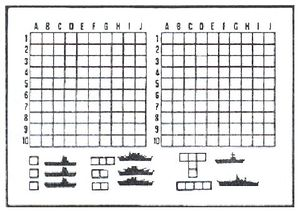
\includegraphics[width=7cm, height=5cm]{Batalhanaval.jpg}
  \centering
  \caption{Clássico Batalha Naval.}
  \label{fig:batalhanaval}
\end{figure}
   
    
    \item \textbf{Clash Royale}\\
    Um jogo [14] que pouco tem em comum com a aplicação desenvolvida, mas que serviu de inspiração para o design e a sua filosofia. O jogo consiste em dois jogadores que têm um exército ao seu dispôr e numa arena, onde estes lutam, dando ordens aos seus exércitos para atacar o outro jogador.
    Neste caso, o jogador tem de escolher a posição onde colocar as suas tropas, sendo que este facto se torna muito importante na mecânica de jogo. 

    A ideia de utilizar um tabuleiro geral para ambos os jogadores, apenas desenhando os \textit{assets} necessários para que cada um veja apenas o necessário em cada momento, veio da interação dos menus do jogo com a mecânica de jogo em si.

\begin{figure}[!h]
  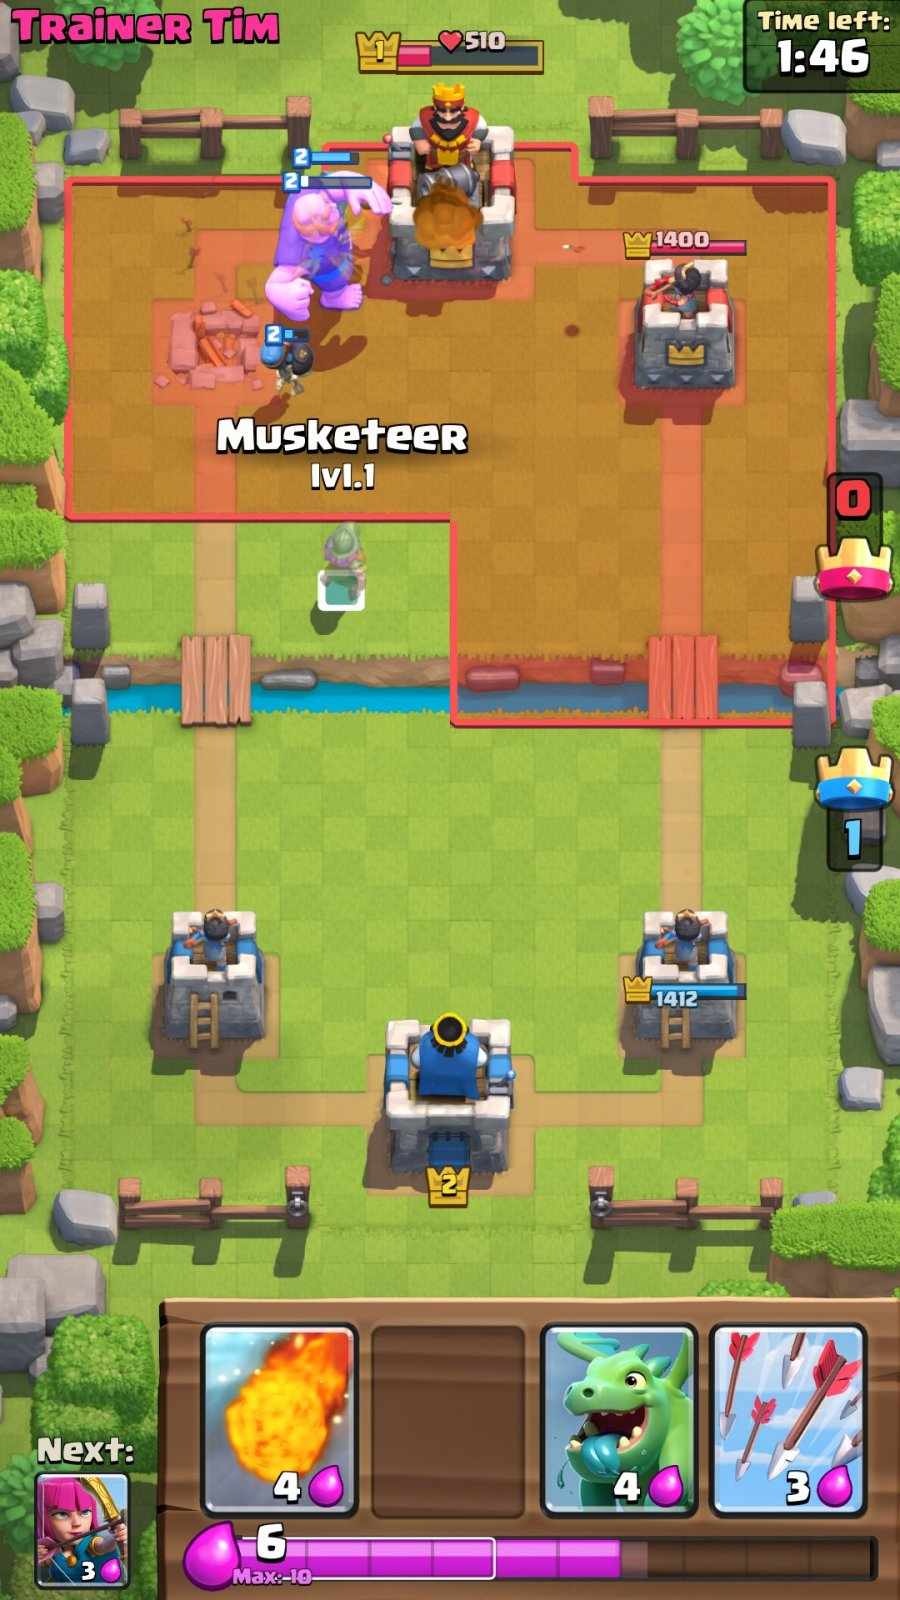
\includegraphics[width=10cm, height=11cm]{clash-royale-4.jpg}
  \centering
  \caption{Ecrã de jogo de uma partida de Clash Royale.}
  \label{fig:clash}
\end{figure}

\end{enumerate}



\clearpage
\section{Conclusões}
\label{chap2:sec:conc}
Com este capítulo, são explicadas as ideias tidas no decorrer do desenvolvimento da aplicação, transmitindo assim uma ideia geral do \textit{mindset} e as bases que foram utilizadas para construir a aplicação. Partindo desta informação, é agora possível avançar para o capítulo referente às \textbf{tecnologias e ferramentas utilizadas} \autoref{chap:tecnologias_ferramentas_utilizadas} no desenvolvimento da aplicação.
\clearpage{\thispagestyle{empty}\cleardoublepage}
\chapter{Tecnologias e Ferramentas Utilizadas}
% OU \chapter{Trabalhos Relacionados}
% OU \chapter{Engenharia de Software}
% OU \chapter{Tecnologias e Ferramentas Utilizadas}
\label{chap:tecnologias_ferramentas_utilizadas}

\section{Introdução}
\label{chap3:sec:intro}
Neste capítulo, são abordadas as ferramentas que foram utilizadas para a construção dos \textit{assets}, assim como também é feito um \textit{overview} do motor de jogo, de maneira a transmitir uma ideia da filosofia e funcionamento geral destas ferramentas.


\section{Blender}
\label{chap3:sec:blender}
Nesta secção, explica-se no que consiste e o processo de criação englobado pela aplicação, apresentando uma opinião pessoal da experiência e aprendizagem com a ferramenta. Expõem-se o trabalho realizado ao utilizar a mesma.

\subsection{Funcionalidades e capacidades}
\label{chap3:subsec:funcionalidades}
Por definição, o \emph{Blender} [4] é uma ferramenta de criação de modelos de computador 3D usada para criar filmes animados, efeitos visuais, modelos para impressão 3D e \textit{assets} para jogos de vídeo.
Inclui funcionalidades para modelação, renderização, rasterização, \textit{rigging} e simulações de corpos físicos complexos, como fumo e fluídos. Compreende um motor de jogo próprio.

\subsection{Experiência}
\label{chap3:subsec:experiencia}
Anteriormente à realização do projeto, o contato com a ferramenta era inexistente. Foi, portanto, necessário um processo de aprendizagem para produzir modelos satisfatórios para uso na aplicação. Esta evolução pode ser notada na crescente qualidade dos modelos, sendo este o pretendido. Desta forma, consegue-se formar uma explicação do processo de evolução que pode ser facilmente entendida e verificada.\\


O primeiro passo passou pela familiarização com a interface da ferramenta e com as funcionalidades que esta apresenta. Após este primeiro passo, foi iniciado o desenvolvimento de formas 3D simples, de modo a perceber várias metodologias para adicionar detalhe e dimensão a estas. Obtendo-se o conhecimento elementar para a produção de modelos com qualidade satisfatória, procedeu-se à produção do primeiro modelo de jogo: o do tanque.

A produção da forma demorou aproximadamente uma semana, uma vez que, ao longo do seu desenvolvimento percebeu-se a necessidade de conhecer mais técnicas de desenho assim como a melhor forma de fazer o \textit{rigging} do modelo.
Sendo assim, estudou-se a melhor maneira de desenvolver gráficos 3D para aplicações móveis onde a máquina destino que vai correr a aplicação pode ter um poder e processamento limitado. As conclusões desse estudo [4] foram as seguintes:
\begin{enumerate}
    \item \textbf{Modelos pouco complexos}, de maneira a simplificar o processo de renderização na máquina destino e, com isto, melhorar o desempenho da aplicação. Um modelo pouco complexo é constituído por formas geométricas simples, como polígonos planos.
    \item \textbf{Formas geométricas simples}, de maneira a haver um número menor de pontos a processar no processo de \textit{render} do modelo, melhorando o desempenho da aplicação. Uma forma geométrica complexa é, por exemplo, uma forma redonda, dado que, para parecer que a sua superfície é suave, precisa de muito tratamento e de ter um número de faces muito elevado (para a resolução utilizada de 800*600 pixeis, seria necessário aproximadamente 34 faces para um cilindro).
    \item \textbf{Evitar \textit{renders} na máquina destino}, sendo que um render em \textit{real-time} é algo muito pesado para um telemóvel fazer. Neste sentido, decidi mudar radicalmente o formato original da aplicação. Em vez de utilizar um sistema dinâmico dos modelos, onde cada modelo é animado no tabuleiro, optou-se por utilizar os modelos para fazer curtas animações em formato vídeo, que seriam depois utilizadas em cada ataque feito por um jogador. Desta maneira, evitou-se fazer \textit{renders} e usa-se apenas um \textit{playback} de um vídeo já produzido, o que aumenta o desempenho da aplicação consideravelmente. 
    \item \textbf{Usar texturas de baixa resolução e pouco complexas}, de maneira a reduzir o impacto no desempenho que a caracterização do modelo tinha.
\end{enumerate}

Tendo em conta estas conclusões, o modelo foi alterado radicalmente, passando de um modelo com um detalhe relativamente elevado para um modelo com aspeto mais quadrado e simples. Esta mudança significou uma melhoria significativa no tempo dos \textit{renders} dos modelos (passando de duas horas para quarenta e cindo minutos). \\

A forma final do modelo, sem tratamento de texturas, iluminação ou pós-produção pode ver-se nas figuras \ref{fig:tanque1}, \ref{fig:tanque2}, \ref{fig:tanque3}, \ref{fig:tanque4} e \ref{fig:tanque5}.

\begin{figure}[!h]
  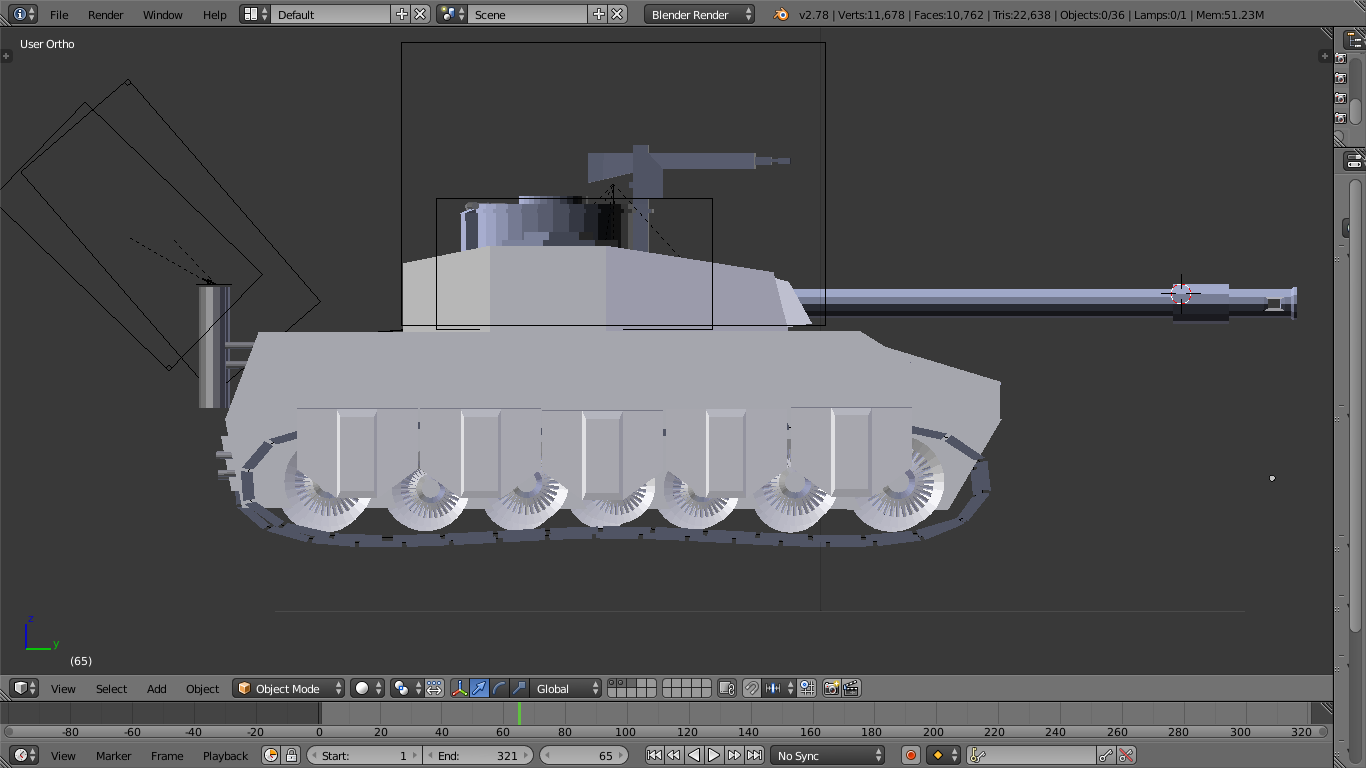
\includegraphics[width=10cm, height=8cm]{p1.png}
  \centering
  \caption{Perfil lateral do modelo do tanque após a modelação.}
  \label{fig:tanque1}
\end{figure}

\begin{figure}[!h]
  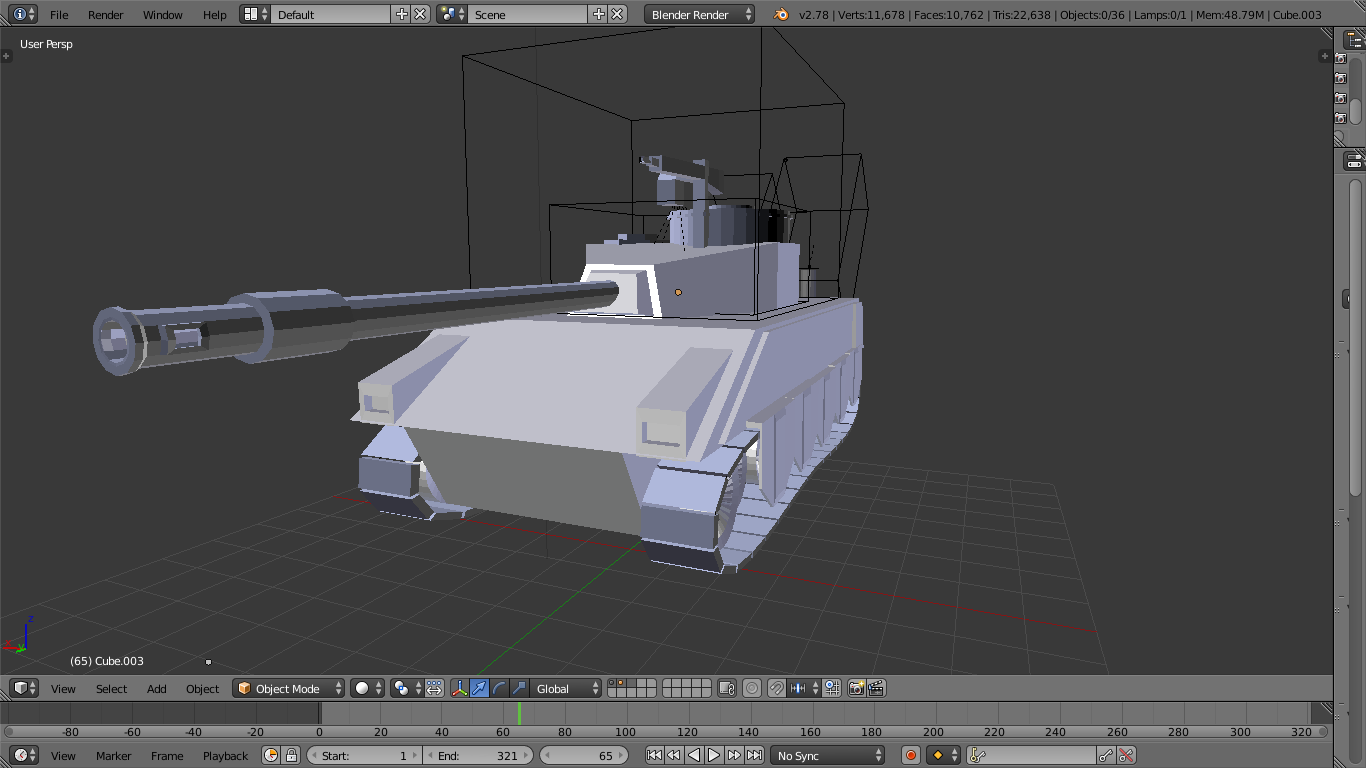
\includegraphics[width=10cm, height=8cm]{p2.png}
  \centering
  \caption{Perfil lateral do modelo do tanque após a modelação.}
  \label{fig:tanque2}
\end{figure}

\begin{figure}[!h]
  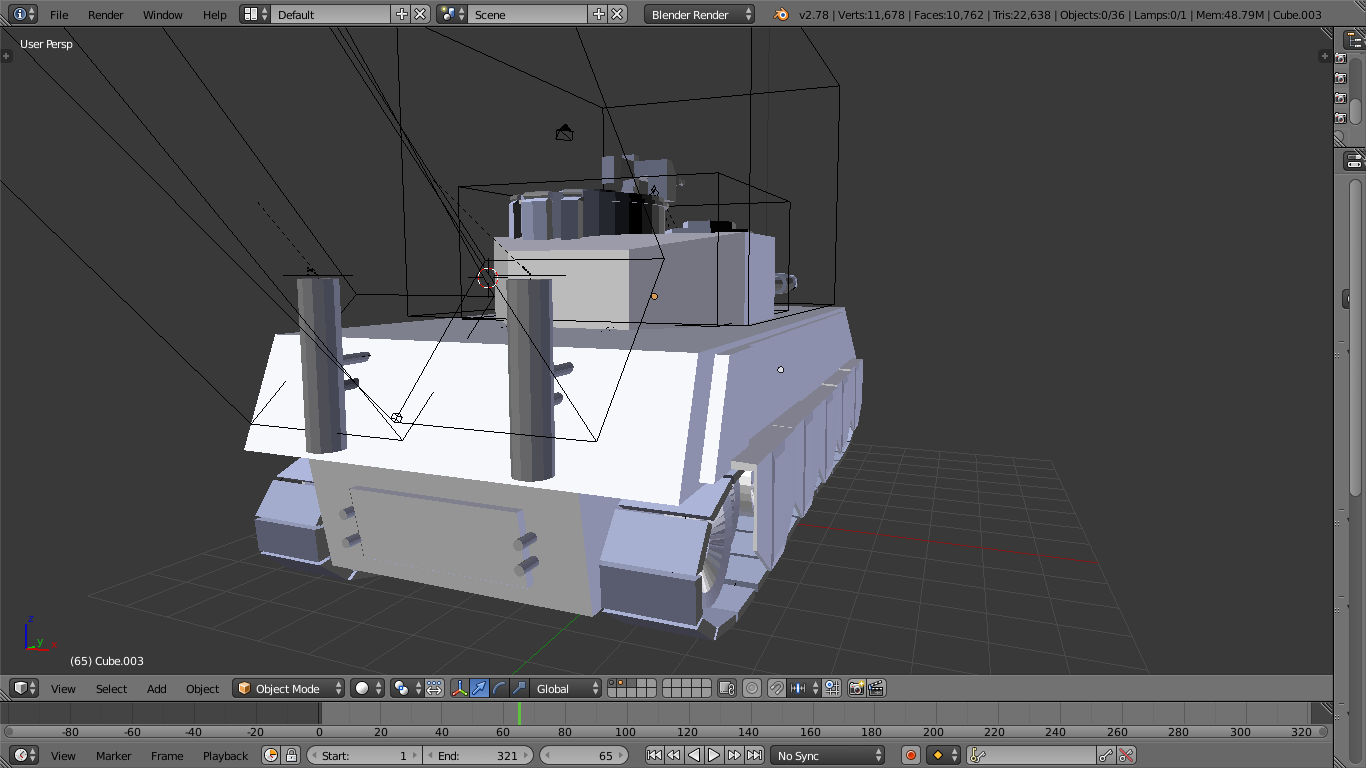
\includegraphics[width=10cm, height=8cm]{p3.png}
  \centering
  \caption{Perfil da retaguarda do modelo do tanque após a modelação.}
  \label{fig:tanque3}
\end{figure}

\begin{figure}[!h]
  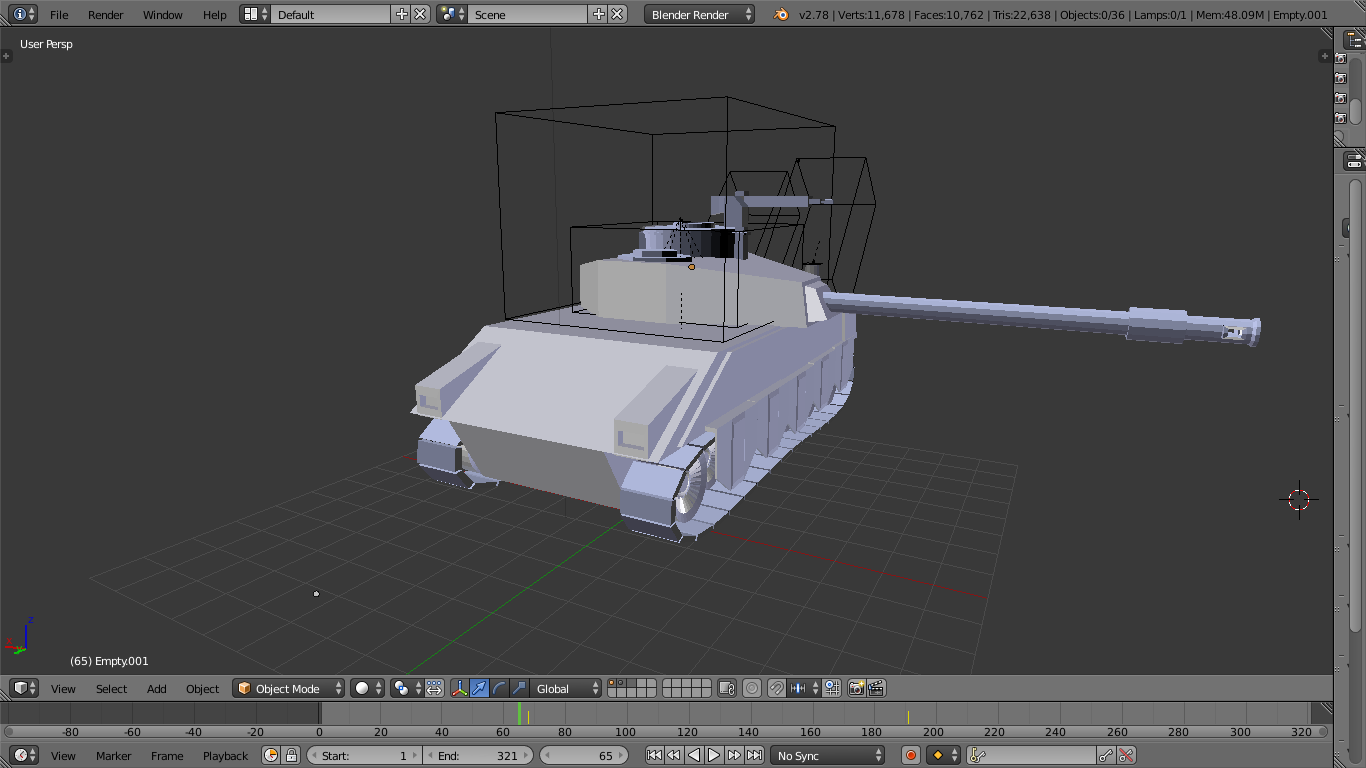
\includegraphics[width=10cm, height=8cm]{p4.png}
  \centering
  \caption{Perfil frontal com a lateral da torre do modelo do tanque após a modelação.}
  \label{fig:tanque4}
\end{figure}

\begin{figure}[!h]
  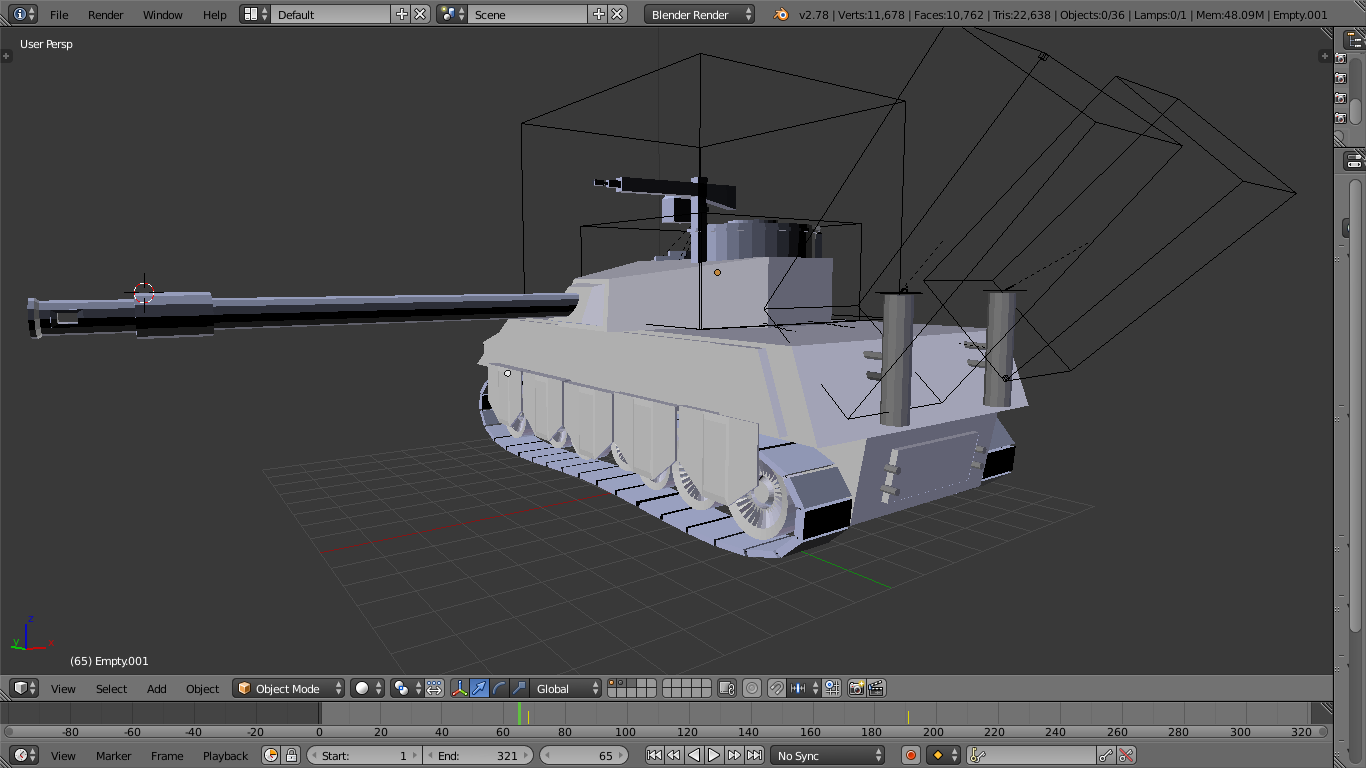
\includegraphics[width=10cm, height=8cm]{p5.png}
  \centering
  \caption{Perfil da retaguarda com a lateral da torre do modelo do tanque após a modelação.}
  \label{fig:tanque5}
\end{figure}

O aspeto visual dos modelos nesta fase de desenvolvimento não difere o suficiente para fazer com que seja necessário mostrar todas estas imagens de perfil para os três modelos, de maneira que apenas são mostradas para o tanque.
Tendo esta forma, procedeu-se a fazer a aplicação de texturas e à iluminação do modelo. \\ 

A aplicação de texturas foi feita de forma simples, usando cores básicas e adicionando apenas algum fator de granularidade nas formas, de maneira a parecer que os modelos tinham uma dimensão de textura que, na realidade, não tinham.
A iluminação foi aplicada usando composição, sendo que o seu ponto inicial, direção e características de força foram alteradas para que nenhuma parte do modelo estivesse escura, mas mantendo a parte frontal mais brilhante que o resto.
Foi então adicionado o fundo, inspirado numa floresta, criado seguindo as guias descritas em cima, referentes aos modelos, utilizado para todos os outros modelos. \\ 

Após esta fase, foi feita a produção dos efeitos de simulação do disparo do veículo e a sua animação (tanto do modelo como dos efeitos de disparo e fumo inseridos). A fase de animação mostrou ser complexa, o que levou a um estudo sobre a matéria. No conjunto, estas quatro fases (aplicação de texturas, iluminação, criação do fundo e animação) demoraram um total de uma semana, sendo que estas não foram tão detalhadas como a fase de modelação. \\ 

Tendo terminado a animação do modelo, foi feita a composição, mais uma vez, de todos os efeitos e iluminação de maneira a refletir o movimento do modelo. Foi então feita a pós-produção do vídeo, adicionando som e corrigindo cores e outros aspetos, de maneira a o tornar mais agradável de ser visualizado. As formas finais dos modelos aqui exibidas foram retiradas dos vídeos que foram produzidos, por isso têm compensação de cor e apresentam algum nível de granularidade, devido à compressão feita para manter os tamanhos dos ficheiros relativamente pequeno.\\ 

A forma final do modelo do tanque, depois de todo o desenvolvimento pode ver-se na figura \ref{fig:fff1}.
\begin{figure}[!h]
  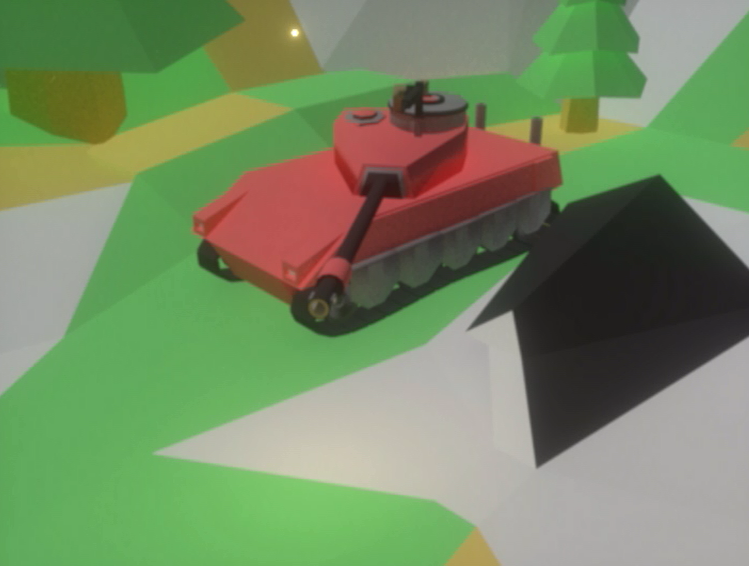
\includegraphics[width=10cm, height=8cm]{model4.png}
  \centering
  \caption{Forma final do modelo do tanque após o seu desenvolvimento.}
  \label{fig:fff1}
\end{figure}

Depois do tanque, foi feito o desenvolvimento do vídeo para uma peça de artilharia. Este desenvolvimento difere do tanque no sentido em que tentei simplificar ainda mais as formas utilizadas, focando mais na animação e composição da aparência depois de modelado. 
Esta abordagem resultou num modelo com uma aparência mais simples, mas que criava a sensação de ser mais complexo que o anterior, especialmente levando em conta os efeitos adicionados depois da modelação.

\clearpage
A forma final do vídeo da artilharia após o seu desenvolvimento pode ver-se na figura \ref{fig:artilharia2}.


\begin{figure}[!h]
 \centerline{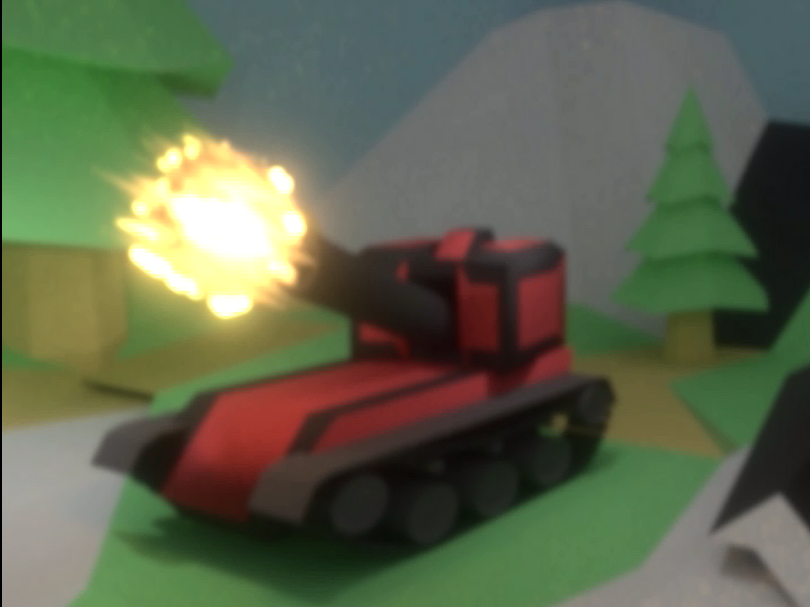
\includegraphics[width=10cm, height=8cm]{model2.png}}
  \centering
  \caption{Forma final do modelo da artilharia após o desenvolvimento.}
  \label{fig:artilharia2}
\end{figure}


Após o desenvolvimento da artilharia, foi iniciado o desenvolvimento do jipe, sendo este o modelo mais complexo e onde o detalhe da composição de efeitos é maior. Por causa disto, é o modelo mais agradável de ver mas também o mais complexo e de maior dimensão em termos de dados, demorando um total de três horas para completar a criação do vídeo (\textit{render} com animação e composição). \\

A forma final do jipe após o desenvolvimento pode ver-se na figura \ref{fig:jipe2}.

Com o desenvolvimento do jipe, acaba a fase em que é usada a ferramenta \emph{Blender}. Após a criação dos modelos e da sua animação é usado o motor de jogo \emph{Unity}, de maneira a os implantar no jogo. 

\begin{figure}[!h]
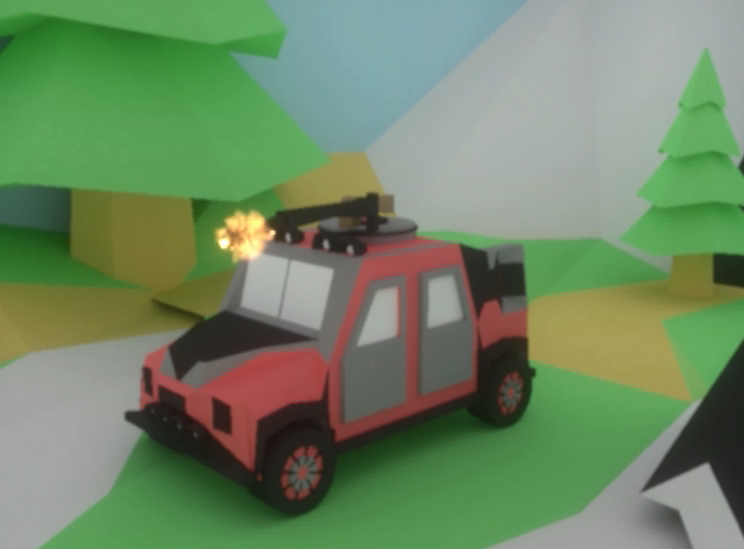
\includegraphics[width=10cm, height=8cm]{model6.png}
  \centering
  \caption{Forma final do modelo do jipe após o desenvolvimento.}
  \label{fig:jipe2}
\end{figure}

Com isto, acaba o desenvolvimento utilizando o \emph{Blender}.
\clearpage
\section{Unity}
\label{chap3:sec:unity}
Nesta secção, vai ser explicado no que consiste a ferramenta \emph{Unity}, as suas funcionalidades e capacidades assim como porque é que é uma opção de qualidade para o desenvolvimento de jogos de vídeo, quer em plataforma móvel quer em plataformas fixas.
\subsection{Funcionalidades e capacidades}
\label{chap3:subsec:funcionalidadesU}
O \emph{Unity} [15] é um motor de jogo \textit{cross-platform} utilizado no desenvolvimento de jogos de vídeo, simulações ou \textit{software} que lide com gráficos complexos. As suas funcionalidades vão desde a visualização de interfaces com gráficos embutidos até modelos de colisão e de física complexos para serem utilizados e gerados a tempo real, tais como simulações de fumo ou fluídos e a inserção de sombras dinâmicas e modelos de iluminação 3D. \\ 

Sendo \textit{cross-platform}, é possível desenvolver aplicações que usam o motor de jogo para um grande número de plataformas, como \emph{Windows}, \emph{Linux}, \emph{Android}, \emph{iOS} e várias consolas.


\subsection{Experiência}
\label{chap3:subsec:experienciaU}
Como aconteceu com a ferramenta Blender, a experiência com a ferramenta Unity era inexistente, onde a necessidade de aprendizagem constitui um fator importante para se conseguir produzir um conteúdo com qualidade satisfatória para ser apresentado na aplicação. Neste caso, a aprendizagem foi um pouco mais rápida que no \emph{Blender}, tendo, mesmo assim, certas dificuldades como a familiarização com a interface, a criação e importação de \textit{assets} e a própria linguagem de programação utilizada para a criação dos \textit{scripts}. Para o processo de aprendizagem, foi utilizado o manual de referência do \emph{Unity} [18]. \\ 

A linguagem de programação escolhida foi \emph{C\#}, sendo que também tinha como opção utilizar \emph{JavaScript}. No entanto, e contado com experiência anterior na utilização de \emph{Java}, foi uma transição relativamente direta para \emph{C\#}, sendo que também se trata de uma linguagem orientada a objetos.

A ligação dos vários componentes gráficos com a mecânica do jogo pretendida é feita através de \textit{scripts}, que são ligados a objetos complexos, chamados \emph{GameObject}'s. Esta ligação permite a utilização de funções e propriedades próprias a um determinado \emph{GameObject} (por exemplo, um \emph{GameObject} do tipo botão tem funcionalidades e propriedades diferentes de um \emph{GameObject} de imagem). \\ 

A utilização da ferramenta foi bastante direta e intuitiva, havendo apenas alguns detalhes que causaram alguns problemas, como o modo de emulação da rede ou as propriedades de visualização da aplicação.

Em termos da ligação entre os dois dispositivos foi feita com base na informação presente na guia de ligações do \emph{Unity} [15].

\section{Conclusão}
\label{chap3:sec:conc}
Com o trabalho desenvolvido neste capítulo, foram aprendidas diversas metodologias e ganhadas várias ideias de como é feito o desenvolvimento de videojogos utilizando as ferramentas referidas, podendo estas experiências traduzir-se em conhecimento que é utilizado em base diária em estúdios de criação da indústria. \\ 
Agora, tendo como base as explicações que foram dadas neste capítulo acerca das funcionalidades e características das ferramentas utilizadas, é possível seguir para a explicação do processo de desenvolvimento da aplicação em si, entrando em mais detalhe na estrutura da aplicação.
\clearpage{\thispagestyle{empty}\cleardoublepage}
\chapter{TankUP - Desenvolvimento}
\label{chap:desen}

\section{Introdução}
\label{chap4:sec:intro}
Neste capítulo é feita uma exposição acerca dos elementos que constituem a aplicação, tal como a sua arquitetura de rede e a dinâmica entre as cenas utilizadas. É exemplificado e explicado o fluxo normal da aplicação, representando um jogo. \\ 
Devido a já terem sido abordadas as etapas nas quais eram incluídas utilizações de ferramentas externas, agora vai ser focado o que está por trás dos \textit{assets}, o que os controla e o que confere conteúdo à aplicação - os \emph{scripts} - formando os pilares do funcionamento de toda a estrutura formada pela conjunção das várias cenas construídas.

De maneira a uma melhor compreensão dos conteúdos apresentados a seguir, é importante ter em conta os seguintes termos: 
\begin{enumerate}
    \item \textit{Scene} - Aqui denominado como cena, é um conjunto de ecrãs da aplicação, sendo que estes ecrãs podem conter várias funcionalidades e gráficos, todos estes ligados através de \textit{scripts}.
    \item \textit{Script} - Agregação de código em \emph{C\#} que confere a capacidade de guardar e manipular informação a um objeto gráfico na cena. Pode estar associado a uma \textit{prefab}.
    \item \textit{Prefab} - Objeto complexo onde é guardada muita informação e funções, aproximando-se a uma classe "dinâmica", que pode interligar outras \textit{prefab}'s, cenas ou objetos. 
\end{enumerate}


\section{Constituição da aplicação}
\label{chap4:sec:TG}
De maneira a conseguir transmitir no que consistiu o processo de desenvolvimento da aplicação, é necessário descrever os seus dois constituintes mais importantes: a \emph{arquitetura de rede} - onde é explicado o funcionamento da comunicação entre os vários componentes de diferentes cenas entre objetos presentes em diferentes dispositivos, implicando comunicação através de rede - e a \emph{dinâmica entre cenas} - onde é demonstrado como é que o bom funcionamento da aplicação depende da interação entre vários objetos presentes em diferentes cenas. \\

De maneira a transmitir melhor a constituição da aplicação, procede-se agora à introdução do seu diagrama de classe \autoref{fig:diagrama}. Como pode ser visto neste, a aplicação é constituída por seis classes principais, que permitem o seu funcionamento. Em termos específicos, os seus propósitos são:
\begin{enumerate}
    \item \textbf{GameManager}: trata do menu na cena \emph{GameMenuScene} e, por isso, instancia e inicia o servidor e os clientes, garantindo depois que os clientes são conectados ao servidor.
    \item \textbf{Server}: aqui são definidos todos os métodos e variáveis que o servidor tem à sua disposição. O servidor vai esperar por ligações, vigiando um \textit{socket}. Quando um cliente se liga a este, vai transmitir a existência dessa ligação para todos os outros clientes e pode agora receber informação desse cliente, sendo essa informação constituída por mensagens codificadas de certa forma, de maneira a que cada uma corresponda a uma funcionalidade do servidor.
    \item \textbf{ServerClient}: quando os clientes são conectados ao servidor, este cria um \textit{ServerClient} para armazenar as informações do cliente, como o seu nome e o facto de este ser o \emph{host} ou não.
    \item \textbf{Client}: os clientes têm vários métodos associados como, por exemplo, a capacidade de enviar informação ao servidor, trabalhar com a informação que recebe do servidor ou criar e controlar um tabuleiro de jogo.
    \item \textbf{GameClient}: sempre que um cliente recebe informação de que um outro cliente também está conectado no servidor, este guarda a informação relativa a esse cliente.
    \item \textbf{MainBoardManager}: age como o controlador do tabuleiro, de maneira a controlar como e onde aparecem os \textit{assets} do jogo, usando também as interfaces do cliente que o criou para enviar directamente informação para o servidor a que o cliente que este está associado está ligado.
\end{enumerate}

\begin{figure}[!h]
    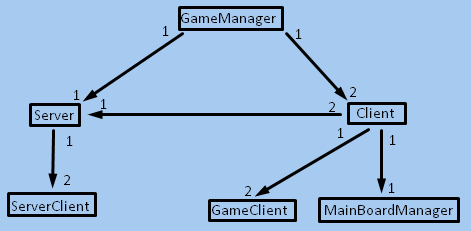
\includegraphics[width=8cm, height=5cm]{Screenshot_1.png}
    \centering
    \caption{Diagrama de classes.}
    \label{fig:diagrama}
\end{figure}

\subsection{Arquitetura de rede}
\label{chap4:subsec:rede}
A \textbf{arquitetura de rede} da aplicação consiste, muito basicamente, em dois clientes e um servidor, sendo que cada cliente tem um tabuleiro próprio e que a comunicação entre clientes é feita por meio do servidor. No entanto, há comunicação entre um cliente e o seu tabuleiro, assim como o tabuleiro consegue aceder a métodos próprios do cliente. 
Mais especificamente, existe uma cena de menu chamada \emph{GameSceneMenu}, onde é implementado um sistema de menu de maneira a que um utilizador possa iniciar um jogo (sendo um \emph{host}) ou juntar-se a um determinado jogo já existente (sendo um \emph{client}).  \\ 

Quando um jogador pressiona o botão \textit{host}, é instanciada uma \textit{prefab} de servidor com o endereço 127.0.0.1 e este é iniciado, ficando então à escuta de possíveis ligações. Também é instanciada uma \textit{prefab} de cliente, dado que o jogador que inicia o servidor também pode jogar, sendo este então conectado ao servidor. Se o jogador desejar conectar-se a um jogo que já foi criado (tendo conhecimento do endereço \ac{IP} local da máquina à qual se deseja conectar), este pode fazê-lo clicando no botão de \emph{Connect} e escrevendo o \ac{IP} da máquina do jogador com o qual este quer jogar.
Neste caso, é instanciada uma \textit{prefab} de cliente e ligada diretamente ao servidor designado pelo endereço \ac{IP} fornecido na caixa presente no menu de conexão do botão \emph{Connect}. \\ 

Quando o servidor é instanciado, este é também iniciado, o que significa que foi aberta uma \textit{socket} \ac{TCP} por onde é possível receber dados, e que o servidor está a escutar este \textit{socket} à procura de mais ligações de clientes.

Quando um cliente se liga ao servidor, este é inserido numa lista de clientes, sendo então registado no servidor com as suas informações básicas (como o seu nome e o facto de ser um \emph{host} ou não). Quando há dois clientes que se ligam a um dado servidor, este pára de escutar ligações novas dá início a uma sessão de jogo. Para fazer isto, o servidor passa as informações de cada cliente para uma lista de jogadores, de maneira a serem facilmente atingíveis. \\ 

A base da comunicação entre clientes e servidores são mensagens constituídas por conjuntos de caracteres, podendo estas gerar combinações que são depois interpretadas pelo destinatário, sendo ainda concatenadas com vária informação relativa ao remetente da mensagem. Desta forma, dependendo da mensagem recebida, diferentes ações vão ser tomadas por ambas as partes. \\ 

A comunicação servidor-cliente é assegurada por uma função de \emph{Broadcast} que envia um conjunto de caracteres para um ou mais objetos do tipo cliente. A comunicação cliente-servidor é, por sua vez, assegurada através da função \emph{Send}, que envia um conjunto de caracteres para o servidor ao qual o cliente se encontra ligado. 



\subsection{Dinâmica entre cenas}
\label{chap4:subsec:dinamica}
O jogo \emph{TankUP} é constituído por várias cenas, formando, em conjunto, todo o conteúdo do jogo que é apresentado ao jogador. Numa cena é tratado um determinado assunto pertinente para a etapa onde a aplicação se encontra num determinado momento, sendo que o tratamento de dados e o \textit{feedback} gráfico da aplicação é dependente dos objetos que estão presentes na presente cena. \\ 
De maneira a manter certa informação entre mudanças de cena, tal como o estado do jogo ou informações dos jogadores conectados ao servidor, é necessário não destruir os dados de determinados elementos da cena anterior. Bons exemplos destes casos são a permanência dos dados relativos ao servidor e aos clientes desde a cena em que são criados até ao final do ciclo de jogo, onde são então destruídos.

Por ordem de aparecimento, as cenas e o seu objectivo geral são:

\begin{table}[!h]
\centering
\caption{Informação acerca das cenas, ordenada por ordem de aparecimento.}

\label{tab:tabela_informacao_cenas}
\begin{tabular}{|c||l|l|}
\hline
\textbf{\#} & \textbf{Nome da cena} & \textbf{Objectivo geral da cena} \\
\hline
\hline
1 & Preloader & Carregamento inicial dos \textit{assets} do jogo \\
\hline	
2 & MenuScene & Menu inicial do jogo \\
\hline
3 & GameMenuScene  & Menu de conexão. Cria servidores e clientes\\
\hline
4 & Board & Tabuleiro onde decorre todo o jogo \\
\hline
\end{tabular}
\end{table}

A informação mais importante da aplicação é criada na cena \emph{GameMenuScene} - Instanciados os clientes e o servidor - e manipulada na cena \emph{Board} - comunicação entre servidor-cliente e cliente-tabuleiro.
A divisão da aplicação nas cenas supramencionadas garante que a sua modularidade, o que permite uma maior facilidade na execução de mudanças ao jogo e à sua manutenção.


\section{Fluxo da aplicação}
\label{chap4:sec:flow}
Nesta secção vai ser representada uma execução normal de um jogo.

\begin{enumerate}
    \item Ambos os jogadores iniciam a aplicação.
    \item Ambos os jogadores clicam o botão \textit{Play} na cena \emph{MenuScene} (\autoref{fig:screen1}).
    \item Ambos os jogadores chegam à cena \emph{GameMenuScene} (\autoref{fig:screen2}).
    \item Um jogador clica o botão de \emph{host} (jogador 1) (\autoref{fig:screen3}) e outro o botão de \emph{connect} (jogador 2) (\autoref{fig:screen4}).
    \item  No jogador 1 é criada uma instância de um servidor, o qual é iniciado, e uma instância de um cliente, a qual é ligada ao servidor criado. No jogador 2 é criada uma instância de um cliente, a qual é ligada ao servidor criado no jogador 1.
    \item Servidor recebe e aceita os pedidos dos jogadores, guardando a informação relativa a cada um. Dado haver dois jogadores conectados em simultâneo, o servidor informa os clientes de que podem mudar para a cena \emph{Board} (\autoref{fig:screen5}), começando o jogo.
    \item No início do jogo, os dois jogadores colocam os seus veículos na posição que desejarem, dentro da sua grelha. No final das colocações, os clientes passam a informação dos tabuleiros construídos ao servidor (\autoref{fig:screen6}).
    \item Quando o servidor recebe a informação dos tabuleiros de cada jogador, este envia uma informação ao jogador 1, com a informação acerca do tabuleiro do jogador 2, e dá-lhe permissão para clicar no botão de ataque. O jogador 2 está à espera.

    \item Quando o jogador 1 clica no tabuleiro, são apresentadas as jogadas anteriores que este fez, onde uma cruz vermelha significa um ataque falhado e um sinal de certo verde indica um ataque com sucesso (\autoref{fig:screen7}). No próximo clique do jogador no tabuleiro, é utilizada essa posição para efetuar um ataque ao jogador 2. O jogador 2 está à espera enquanto isto acontece. 
    \item Depois de escolhido o ataque, este é validado e enviado ao servidor se respeitar as regras do jogo. É então revogada a permissão do jogador 1 poder atacar e esta é dada ao jogador 2. Quando isto acontece, o seu tabuleiro é desenhado outra vez, de maneira a refletir o ataque que sofreu, com uma cruz vermelha na posição atacada (\autoref{fig:screen8}). O jogador 1 está à espera.
    \item Este ciclo de ataque e espera é repetido até que um dos jogadores consiga destruir todos os veículos inimigos, sendo então mostrada uma mensagem a ambos os jogadores com o vencedor.
    \item Jogo termina e ambos os jogadores são reencaminhados para a cena \emph{GameMenuScene}. 
\end{enumerate}
 
 \begin{figure}[!h]
    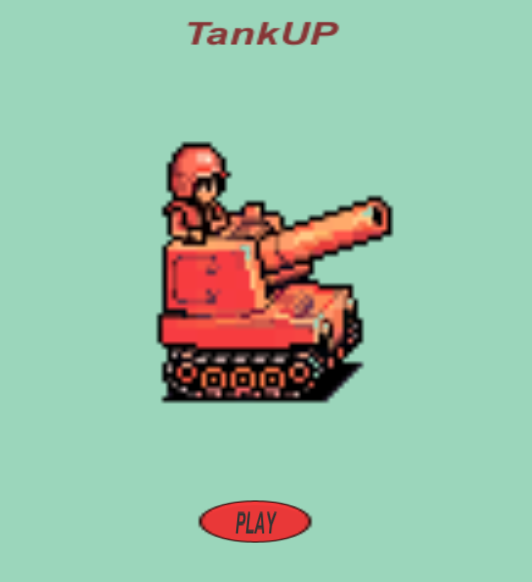
\includegraphics[width=10cm, height=8cm]{sceen1.png}
    \centering
    \caption{Cena MenuScene}
    \label{fig:screen1}
\end{figure}

\begin{figure}[!h]
    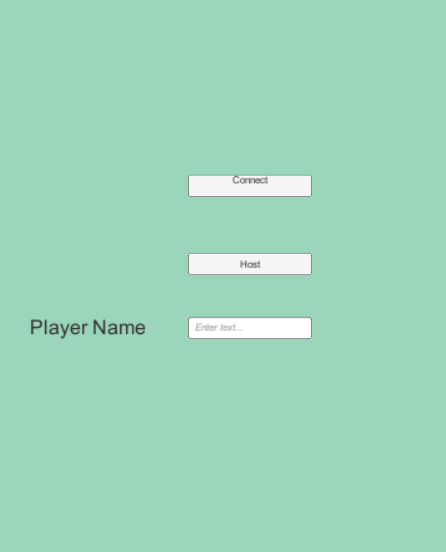
\includegraphics[width=10cm, height=8cm]{screen2.png}
    \centering
    \caption{Cena GameMenuScene}
    \label{fig:screen2}
\end{figure}

\begin{figure}[!h]
    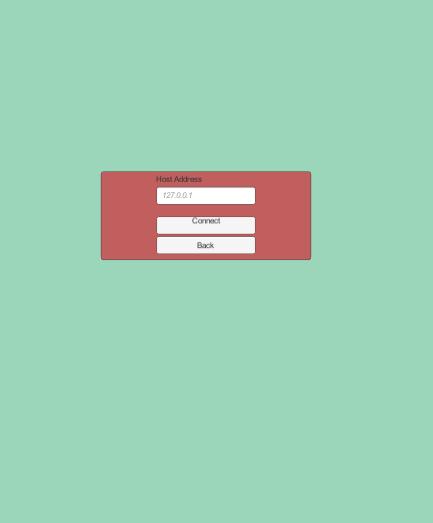
\includegraphics[width=10cm, height=8cm]{screen3.png}
    \centering
    \caption{GameMenuScene com seleção de host.}
    \label{fig:screen3}
\end{figure}

\begin{figure}[!h]
    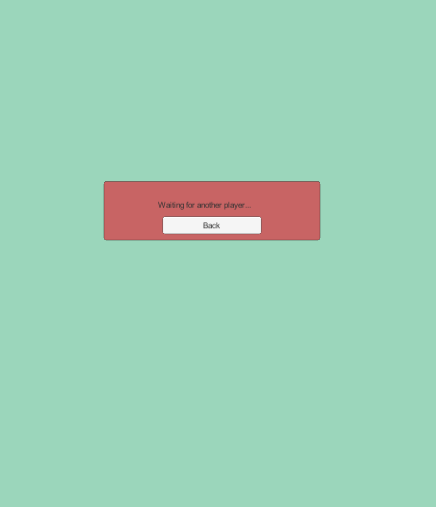
\includegraphics[width=10cm, height=8cm]{screen4.png}
    \centering
    \caption{GameMenuScene com seleção de conexão.}
    \label{fig:screen4}
\end{figure}
    
\begin{figure}[!h]
    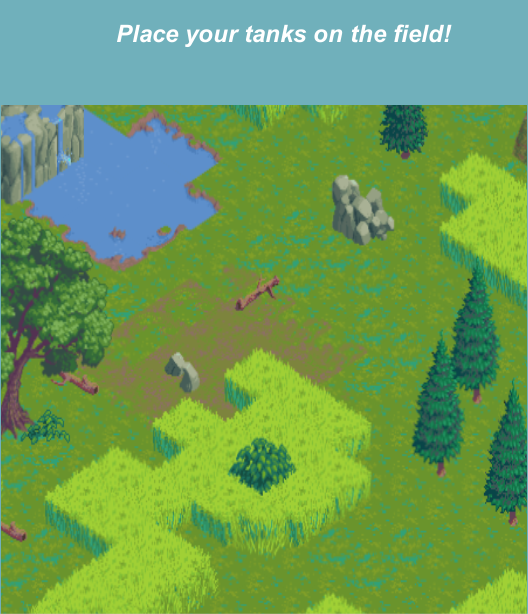
\includegraphics[width=10cm, height=8cm]{screen6.png}
% * <individuoamaral@gmail.com> 17:26:12 07 Jul 2017 UTC+0100:
% ALTERAR IMAGEM
    \centering
    \caption{Cena Board.}
    \label{fig:screen5}
\end{figure}
    
\begin{figure}[!h]
    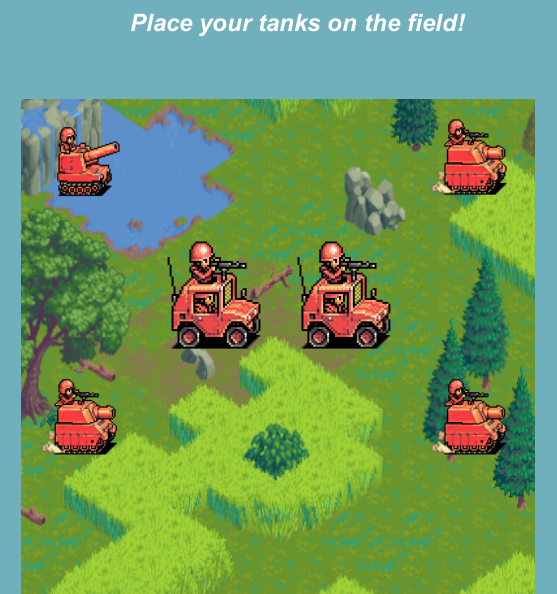
\includegraphics[width=10cm, height=8cm]{screen5.png}
    \centering
    \caption{Cena Board com veículos colocados.}
    \label{fig:screen6}
\end{figure}

\begin{figure}[!h]
    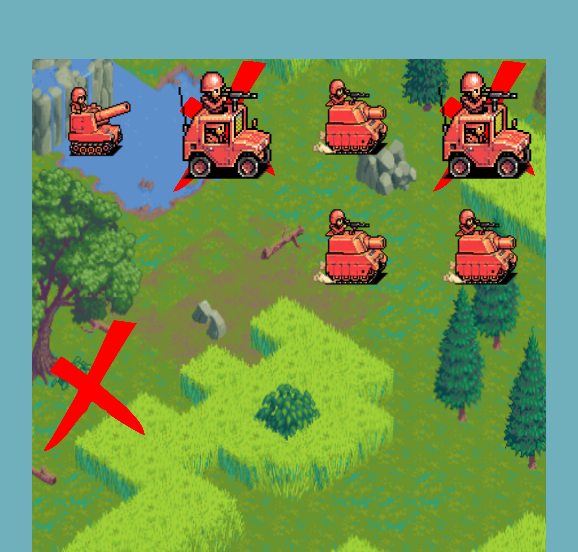
\includegraphics[width=10cm, height=8cm]{screen7.png}
    \centering
    \caption{Cena Board com ataques efectuados.}
    \label{fig:screen7}
\end{figure}

\begin{figure}[!h]
    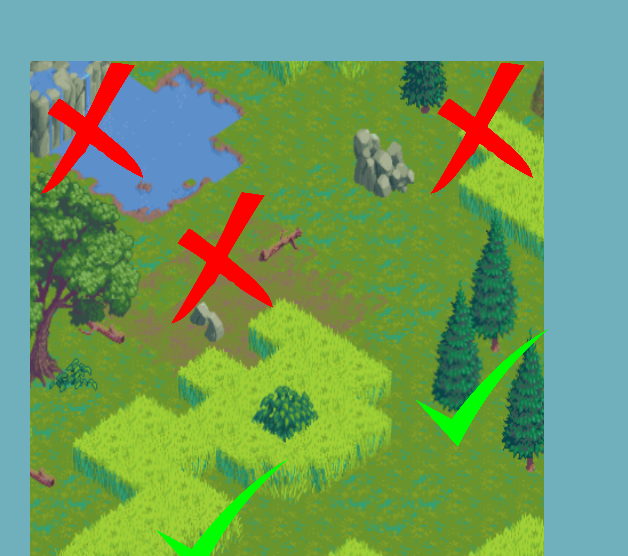
\includegraphics[width=10cm, height=8cm]{screen8.png}
    \centering
    \caption{Cena Board com veículos colocados e ataques sofridos.}
    \label{fig:screen8}
\end{figure}
    
\clearpage
Assim termina uma partida de \emph{TankUP}.

Em termos da integração do jogo na plataforma \emph{Android}, houveram algumas dificuldades de compatibilidade, devido a definições de \textit{build} erradas. Para ajudar na integração, assim como no \textit{playback} dos vídeos feitos no \emph{Blender}, usou-se o manual de referência do \emph{Android} [9].

\section{Conclusão}
\label{chap4:sec:conc}
Neste capítulo foram transmitidas as características dos constituintes mais importantes da aplicação: a \emph{arquitetura de rede} \autoref{chap4:subsec:rede} - criados dois clientes e um servidor, que vai estar a escutar uma \textit{socket} à procura de novas ligações de clientes, sendo que os dois clientes vão ser ligados a este, possibilitando assim comunicação servidor-cliente - e a \emph{Dinâmica entre cenas} \autoref{chap4:subsec:dinamica} - são criados vários objetos em diferentes cenas que têm de ser mantidos de maneira a não perder qualquer informação importante gerada numa cena passada. Com este entendimento acerca deles, é possível acompanhar um desenvolvimento de uma partida de \emph{TankUP}, como a que foi representada em \autoref{chap4:sec:flow}, estando assim completo o ciclo de vida da aplicação e, por isso, o ciclo de desenvolvimento de conteúdo. \\

A seguir, serão referidos trabalhos futuros, assim como melhorias que poderiam ser implementadas na aplicação de maneira a aumentar a sua qualidade. É também feita uma conclusão para as temáticas abordadas neste relatório e, por isso, na aplicação.
\clearpage{\thispagestyle{empty}\cleardoublepage}
\chapter{Conclusões e Trabalho Futuro}
\label{chap:futuroC}

\section{Introdução}
\label{chap7:sec:intro}
Neste capítulo vão ser abordados trabalhos futuros na aplicação ou utilizando a aplicação como base, tais como o refinamento do conteúdo já presente, o desenvolvimento de conteúdo extra ou utilização do código para a criação de uma nova aplicação. Além disto, é feita uma conclusão acerca de todo o processo de desenvolvimento, transmitindo assim as ideias mais importantes que seria de maior importância reter acerca do desenvolvimento da \emph{TankUP}.


\section{Conclusão}
\label{chap7:sec:conc}
Em termos do desenvolvimento da aplicação, foram conseguidos todos os objetivos pretendidos, formando assim uma aplicação completa e que consegue englobar as grandes áreas do desenvolvimento de jogos.\\

Neste processo de criação foram ultrapassadas muitas dificuldades, como a aprendizagem das ferramentas, a conexão dos modelos com o motor de jogo, a conexão dos clientes com o servidor, o controlo do tabuleiro por parte de um cliente, comunicar do tabuleiro para o servidor e até a compatibilidade da aplicação com a plataforma \emph{Android}, que é suposto ser garantida pelo motor de jogo \emph{Unity}.
Para resolver estes problemas, foram consultados vários guias, mencionados na bibliografia. 

No entanto, com a realização deste projeto, foi possível aprender novos conceitos, tais como modelação, animação, design gráfico e elementos de pós-produção, e também foi possível melhorar os meus conhecimentos de ligações de rede, de programação orientada a objetos e de engenharia de \textit{software}.\\

A área do desenvolvimento de videojogos consegue englobar uma grande diversidade de conceitos fundamentais no contexto da engenharia informática, como pode ser constatado no desenvolvimento do \emph{TankUP}, formando, na minha perspectiva, um excelente tipo de projeto, uma vez que consegue conjugar um certo fator de divertimento, um interesse pessoal e uma área que se encontra em grande desenvolvimento e expansão com elementos académicos.

O desenvolvimento de jogos é uma área da informática cada vez mais disponível para o público geral, sendo possível e, na minha opinião, muitas vezes indicado que este desenvolvimento se encare como um possível meio de distribuição de conhecimento a qualquer público interessado na área de engenharia informática.

\section{Trabalho futuro e melhorias}
\label{chap7:sec:tfm}

\subsection{Refinamentos}
\label{chap7:subsec:EF}
A primeira fase de trabalhos futuros passaria por refinar a aparência e funcionamento da aplicação, de maneira a melhorar a experiência do utilizador, aumentando a qualidade da aplicação.
Esta seria a fase mais custosa e de maior duração, dado que a manutenção e melhoramento da aplicação é um processo contínuo e que tem de ser reavaliado sempre que qualquer conteúdo é adicionado e que começa logo que o processo de desenvolvimento principal da aplicação é terminado

Especificamente, na fase inicial de refinamento seria necessário resolver ou melhorar os seguintes aspetos:
\begin{enumerate}
    \item Refazer os modelos aumentando o número de polígonos, de maneira a conferir aos modelos um aspeto mais aprimorado e menos quadrado.
    \item Criar e aplicar texturas de camuflagem e de desgaste aos modelos dos veículos.
    \item Criar animações e vídeos de maior qualidade, usando tecnologias mais avançadas para a construção de cinemáticas mais realistas.
    \item Implementar um sistema de procura de partidas, de maneira a que um jogador não tenha de saber o endereço \ac{IP} de uma máquina \textit{host} para jogar.
    \item Implementar um sistema de \textit{chat} entre os dois jogadores.
    \item Implementar um tabuleiro com modelos 3D, substituindo a vista \textit{top-down} que o jogo apresenta.
    \item Melhorar o sistema de comunicação entre o cliente e o servidor, de maneira a enviar menos mensagens pela rede. 
\end{enumerate}

Com as melhorias mencionadas acima implementadas, é expectável que a qualidade da aplicação suba consideravelmente, sendo mais confortável e agradável de ser utilizada por qualquer jogador.

\subsection{Conteúdo Extra}
\label{chap7:subsec:CE}
Um dos pontos onde a indústria dos videojogos está a apostar fortemente é em conteúdo novo que é desenvolvido para um jogo já existente, adicionando novas camadas de complexidade e interesse. Este conteúdo, referido na indústria como \ac{DLC}, pode conferir um interesse e uma dimensão completamente renovada a um jogo que já tenha alguma idade, mantendo-o relevante por mais tempo. 
Este tipo de conteúdo tem várias vantagens do que simplesmente produzir um novo jogo, como por exemplo:
\begin{enumerate}
    \item O custo relacionado a produzir conteúdo para um jogo já existente é consideravelmente menor do que produzir um novo jogo de raiz.
    \item O esforço criativo de criar conteúdo para um jogo que já tem uma ideia de conteúdo fixa é muito mais baixo que criar um novo universo de jogo, com significados, contextos e conteúdos novos. Esta ideia também se aplica a sequelas.
    \item Quando um jogo é bem-sucedido, quer dizer que o seu público gostou das ideias que foram usadas para o desenvolver. Esse facto pode ser aproveitado para fazer sequelas ou conteúdo relativamente parecido com  o conteúdo original, o que é provável ter um sucesso comparável com o o que foi desenvolvido anteriormente.
\end{enumerate} 

Todo este conteúdo podia ser disponibilizado gratuitamente ao público ou requerer uma pequena taxa por parte dos jogadores, o que poderia servir para financiar o desenvolvimento de mais e melhor conteúdo.

 \subsection{Criação de uma nova aplicação}
\label{chap7:subsec:CA}
Todo o conhecimento que foi adquirido na construção desta aplicação pode ser adaptado para a produção de outros programas, com funcionalidades e objetivos radicalmente diferentes, tais como aplicações de comunicação ou com interfaces gráficas complexas. Um exemplo seria uma aplicação de comunicação entre os operários de uma fábrica e os responsáveis por abastecer os operários de materiais que usam em construções, podendo usar uma interface gráfica com modelos 3D dos materiais, de maneira a facilitar a sua identificação por parte de operadores que podem não ter treino ou capacidade de controlar uma aplicação mais complexa ou convoluta. \\ 

 Devido à modularidade que a aplicação \emph{TankUP} apresenta e, levando em conta as funcionalidades de que o motor \emph{Unity} dispõe, uma adaptação da aplicação para um propósito semelhante ao referido acima não seria uma tarefa demasiado complexa.

\clearpage{\thispagestyle{empty}\cleardoublepage}



% SE EXISTIREM APENDICES, DESCOMENTAR O QUE ESTÁ EM BAIXO
% \appendix
% \include{apendice1}
% \clearpage{\pagestyle{empty}\cleardoublepage}
% \include{continuacao}
% \clearpage{\pagestyle{empty}\cleardoublepage}
% \include{apendice2}
% \clearpage{\pagestyle{empty}\cleardoublepage}
% \include{apendice3}
% \clearpage{\pagestyle{empty}\cleardoublepage}

\backmatter
\chapter{Bibliografia}
\label{Bibliografia}

\quad [1] APPLE (2017). \textit{Iphone SDK}.  Disponível em: \url{http://developer.apple.com/iphone/}. \\

[2] Arneson, Erik (2017). \textit{Salvo - Complete Rules for Battleships Game}.  Disponível em: \url{https://www.thespruce.com/g00/salvo-complete-rules-412378?i10c.referrer=https\%3A\%2F\%2Fen.wikipedia.org\%2F}. \\

[3] Bawa, Mayank \textit{et. al.}. \textit{Peer-to-Peer Research at Stanford}. Consultado a 11 Fevereiro 2017. Disponível em: \url{http://www.cc.gatech.edu/~mihail/D.8802readings/garciamolina1.pdf}. \\

[4] Blain, Jonh (2016).  \textit{The Complete Guide to Blender Graphics : Computer Modeling \& Animation}. 3(1). Publicado por: \textit{Taylor \& Francis Inc}.  \\

[5] Blender (2017). \textit{About}.  Disponível em: \url{https://www.blender.org/about/}. \\

[6] Bluetooth (2017). \textit{What is Bluetooth?}. Consultado a 12 Fevereiro 2017. Disponível em: \url{https://www.bluetooth.com/what-is-bluetooth-technology/how-it-works}. \\

[7] Chemini, F., Coulton, P., e Edwards, R. (2008). Evolution of 3d mobile games development.
\textit{Personal Ubiquitous Comput}, 12(1), 19–25. \\

[8] Epstein, Eli \textit{et. al.}. \textit{The Evolution of Gaming}. Concultado a 14 Fevereiro 2017. Disponível em: \url{http://mashable.com/2015/01/08/gaming-tech-ces/#sUvIKe26Ysql}. \\

[9] Google (2017). \textit{Android Reference Manual}. Consultado a 6 Fevereiro 2017. Disponível em \url{https://developer.android.com/reference/packages.html}. \\

[10] IDC (2016). \textit{Smartphone OS Market Share, 2016 Q3}. Consultado a 22 Fevereiro 2017. Disponível em \url{http://www.idc.com/promo/smartphone-market-share/os}. \\

[11] Joselli, Mark e Clua, Esteban (2009). \textit{Mobile Game Development: A Survey on the Tecnology and Platforms for Mobile Game Development}. Consultado a 14 Fevereiro 2017. Disponível em: \url{https://mjoselli.files.wordpress.com/2012/12/mobilevideojogos09.pdf}. \\

[12] Klement, Scott (s.d.). \textit{Introduction to TCP and Sockets}.  Consultado a 10 Fevereiro 2017. Disponível em: \url{https://www.scottklement.com/rpg/socktut/introduction.html}. \\

[13] Microsoft (2017). \textit{C\# Programming Guide}. Consultado a 23 Abril 2017. Disponível em: \url{https://docs.microsoft.com/en-us/dotnet/csharp/programming-guide/index}. \\

[14] Suppercell (2017). \textit{Clash Royale Battle - Basic Rules}.  Disponível em: \url{http://clashroyalearena.com/guides/clash-royale-battle-basic-rules}. \\

[15] Unity (2017). \textit{Network Clients and Servers}. Concultado a 24 Abril 2017. Disponível em: \url{https://docs.unity3d.com/Manual/UNetClientServer.html}. \\

[16] Unity (2017). \textit{Unity 3D Game Engine}. Disponível em: \url{http://unity3d.com/}. \\

[17] Unity (2017). \textit{Public Relations}. Consultado a 15 Fevereiro 2017. Disponível em \url{https://unity3d.com/public-relations}. \\

[18] Unity (2016). \textit{Unity Manual}. Consultado a 20 Abril 2017. Disponível em: \url{https://docs.unity3d.com/560/Documentation/Manual/}. \\















\include{bibliography}


\end{document}